\chapter{3Dプログラミングへの挑戦}
\section{モデルの回転} \label{sec:06-rotate}
\begin{itembox}[l]{原点を通る\(y\)軸回転}
\begin{verbatim}
 1: #include <FK/FK.h>
 2: 
 3: int main(int, char **)
 4: {
 5:     fk_AppWindow    window;
 6:     fk_Block        block(10.0, 10.0, 10.0);
 7:     fk_Model        modelA, modelB;
 8:     fk_Vector       origin(0.0, 0.0, 0.0);
 9: 
10:     modelA.setShape(&block);
11:     modelA.setMaterial(Yellow);
12:     modelA.glMoveTo(20.0, 20.0, 0.0);
13:     window.entry(&modelA);
14: 
15:     modelB.setShape(&block);
16:     modelB.setMaterial(Red);
17:     modelB.glMoveTo(20.0, -20.0, 0.0);
18:     window.entry(&modelB);
19: 
20:     window.setSize(800, 600);
21:     window.setBGColor(0.6, 0.7, 0.8);
22:     window.open();
23: 
24:     while(window.update() == true) {
25:         modelA.glRotate(origin, fk_Y, FK_PI/180.0);
26:         modelB.glRotateWithVec(origin, fk_Y, FK_PI/180.0);
27:     }
28:     return 0;
29: }
\end{verbatim}
\end{itembox}
\subsection*{解説}
\begin{itemize}
 \item 8行目では、fk\_Vector型(ベクトル)の変数宣言の際に、
	引数に3個の実数を入力しています。
	fk\_Vector型では、このように記述しておくと変数宣言時に
	ベクトルの初期値設定が可能です。「origin」というのは
	「(数学的な意味での)原点」という意味の英単語で、
	原点を表すベクトル変数の名称としてよく用いられます。
	(もっと略して「org」とすると、「original」と混同して
	しまって若干紛らわしくなります。)

 \item 25,26行目にある「glRotate()」と「glRotateWithVec()」という関数は、
	共にモデルに対して回転移動を行います。
	3次元での回転は、「回転軸」と「角度」を指定することになります。
	(両者の違いは次の項目で述べます。)

	回転軸の指定の仕方は色々あるのですが、
	今回は「回転軸が通る点」と「回転軸に平行な座標軸」という
	指定の方法を用いています。

	最初の引数となっている「origin」が回転軸が通る点で、
	「fk\_Y」は「\(y\)軸に平行な回転軸」ということになります。
	結果的に、今回は共に\(y\)軸そのものを中心に
	回転していることになります。

	3番目の引数角度は「弧度法(ラジアン)」という、\(2\pi\)を1回転とする
	角度単位で指定します。29行目にある「FK\_PI」というのは
	FKのプログラム中で用いることができる円周率\(\pi\)を意味します。
	従って、今回のループ1回あたりの回転角は\(\frac{\pi}{180}\)(rad)で、
	これは度数法でいう\(1^{\circ}\)となります。

 \item glRotate() 関数と glRotateWithVec() 関数は共にモデルの回転移動を
	行うものですが、glRotate() の方はあくまで物体の位置のみを変化
	させるもので、物体の向きについては変更を行いません。
	それに対し、glRotateWithVec() は位置の移動と共に向きも回転します。
	用途によって使い分けて下さい。

\end{itemize}

\section{ローカル座標系} \label{sec:06-local}
\begin{itembox}[l]{グローバル回転とローカル回転}
\begin{verbatim}
 1: #include <FK/FK.h>
 2: 
 3: int main(int, char **)
 4: {
 5:     fk_AppWindow    window;
 6:     fk_Block        block(10.0, 10.0, 10.0);
 7:     fk_Model        modelA, modelB;
 8:     fk_Vector       origin(0.0, 0.0, 0.0);
 9: 
10:     modelA.setShape(&block);
11:     modelA.setMaterial(Yellow);
12:     modelA.glMoveTo(20.0, 0.0, 0.0);
13:     window.entry(&modelA);
14: 
15:     modelB.setShape(&block);
16:     modelB.setMaterial(Red);
17:     modelB.glMoveTo(20.0, 0.0, 0.0);
18:     window.entry(&modelB);
19: 
20:     window.setSize(800, 600);
21:     window.setBGColor(0.6, 0.7, 0.8);
22:     window.open();
23: 
24:     while(window.update() == true) {
25:         modelA.glRotateWithVec(origin, fk_Y, FK_PI/180.0);
26:         modelB.loRotateWithVec(origin, fk_Y, FK_PI/180.0);
27:     }
28:     return 0;
29: }

\end{verbatim}
\end{itembox}
\subsection*{解説}
\begin{itemize}
 \item ここでは、「\textbf{グローバル座標系}」と「\textbf{ローカル座標系}」と
	呼ばれる概念を説明します。
	これまで、位置や方向を表す「座標軸」というのは
	プログラムの仮想世界の中では一つだけであり、不動のものでした。
	これに対し、各モデルの中心を原点とし、
	各モデルの向いている方向によって
	規定される座標系を「ローカル座標系」と言います。
	図\ref{Fig:06-Local}にその概念図を示します。
	\(xy\)がグローバル座標系、\(x'y'\)がローカル座標系です。
	\begin{figure}[H]
	\centering
	\includegraphics[width=5cm]{./Fig/Fig06-01.eps}
	\caption{グローバル座標系とローカル座標系}
	\label{Fig:06-Local}
	\end{figure}
	fk\_Model では多くの移動や方向指定の関数に、
	グローバル座標系とローカル座標系用の両方の関数が用意されています。
	グローバル座標系は、現在のモデルの位置や方向に従わないような
	指定、現実世界では「東西南北」を基本とした指定に向いています。
	一方のローカル座標系での指定は、モデル自身を中心とした指定、
	すなわち「前後左右」を基本とした指定に向いています。

\item 26行目にある「loRotateWithVec()」関数は、ローカル座標系による
	回転移動を行うものです。27行目の glRotateWithVec() と同じく
	原点を通る\(y\)軸回転を行っていますが、
	ローカル座標系の場合はモデルの中心がそのまま原点となりますから、
	modelB は同じ場所に留まって回転します。
	一方で modelA は(グローバル座標系の)原点を中心に回転していきます。

\item 平行移動にも glTranslate() と対となる
	「loTranslate()」関数があります。例えば fk\_Model 型の変数
	「model」があったとして、
	\begin{screen}
	\begin{verbatim}
	model.glTranslate(0.0, 0.0, -1.0);
	\end{verbatim}
	\end{screen}
	はモデルがどちらを向いていようが \((0, 0, -1)\) だけ平行移動しますが、
	\begin{screen}
	\begin{verbatim}
	model.loTranslate(0.0, 0.0, -1.0);
	\end{verbatim}
	\end{screen}
	の場合は物体の向いている方向に前進します。
	(FKでは\((0, 0, -1)\)が物体の前方向を意味します。)
	
\end{itemize}

\section{カメラの移動} \label{sec:05-camera}
\begin{itembox}[l]{カメラモデルの制御}
\begin{verbatim}
 1: #include <FK/FK.h>
 2: 
 3: int main(int, char **)
 4: {
 5:     fk_AppWindow    window;
 6:     fk_Model        camera;
 7:     fk_Vector       origin(0.0, 0.0, 0.0);
 8: 
 9:     camera.glMoveTo(0.0, 1.0, 0.0);
10:     window.setCameraModel(&camera);
11:     window.showGuide(FK_GRID_XZ);
12:     window.setSize(800, 600);
13:     window.setBGColor(0.6, 0.7, 0.8);
14:     window.open();
15: 
16:     while(window.update() == true) {
17:         if(window.getSpecialKeyStatus(FK_UP) == FK_SW_PRESS) {
18:             camera.loTranslate(0.0, 0.0, -0.1);
19:         }
20: 
21:         if(window.getSpecialKeyStatus(FK_LEFT) == FK_SW_PRESS) {
22:             camera.loRotateWithVec(origin, fk_Y, FK_PI/180.0);
23:         }
24:     }
25:     return 0;
26: }
\end{verbatim}
\end{itembox}
\subsection*{解説}
\begin{itemize}
 \item このサンプルプログラムでは、これまでのように形状を作成する
	型が何も用いられていません。そのかわり、
	11行目にあるfk\_AppWindow型変数での\\
	「showGuide()」という関数が記述されています。
	この関数は、仮想世界上に
	「グリッド」という格子状の線を表示するためのもので、
	今回は\(xz\)平面に沿ってグリッドが作成されます。

 \item 10行目の「setCameraModel()」という関数は、
	ある fk\_Model型の変数を\&記号を付けて引数として入力することで、
	そのモデルを仮想世界上の「カメラ」となるように設定する関数です。
	これまで FK プログラムのカメラは不動のものでしたが、
	このモデルを中心に一人称視点で仮想世界上を動き回るプログラムを
	作成することができます。

 \item 18行目では、前節の解説で説明した「loTranslate()」関数が
	用いられています。27行目でカメラが回転した場合でも、
	ローカル座標系による指定なので上矢印キーが押された場合は
	常に前進(\((0, 0, -0.1)\)の平行移動)するようになっています。

\end{itemize}

\section{練習課題} \label{sec:06-q}
\begin{description}
 \myitem \ref{sec:05-camera}節のプログラムに対し、下矢印キーで後退、
	右矢印キーで右回転する機能を追加せよ。

 \myitem 上記のプログラムに対し、建物に見立てた形状を空間内に配置し、
	街中を動き回るようなプログラムを作成せよ。

 \myitem さらに上記のプログラムに対し、
	作成した建物をすり抜けないような処理を追加せよ。
\end{description}
